%----------------------------------------------------------------------------
\chapter{Mérések}
\label{sec:results}
%----------------------------------------------------------------------------

A következő fejezetben szeretném bemutatni, hol és hogyan készültek a mérési eredmények, azokból mi olvasható ki. Fontos megjegyezni, hogy komolyabb mérések még a diplomamunka hátralevő részére vannak ütemezve, az alább bemutatott eredmények a rendszer működőképességét igazolják és némi előretekintést nyújtanak.

%----------------------------------------------------------------------------
\section{Mérés környezete}
%----------------------------------------------------------------------------
A feladat elején főként implementációval kellett foglalkozni így nem kapott jelentős szerepet a Kubernetes klaszter. Ezért  a félév első felében elég volt lokálisan futtatni, amit én Minikube (v1.17.1) segítségével tettem meg. 

Amikor a fejlesztési rész kezdett véglegesedni kellett egy rendes környezet, a rendes mérésekhez. Ehhez több lehetőséget is számításba vettem.	

\begin{itemize}
  \item \textbf{BME Cloud}: Egyik lehetőség az egyetemi felhő volt. Itt létre lehet hozni virtuális gépeket, amiket aztán klaszterbe lehet szervezni. Hátránya viszont, hogy hosszabb távra nehezen lehet gépet igényelni, rendszeresen le is állítják ami könnyen okozhatja egy-egy mérés elvesztését, hiszen több órán keresztül is futhat.
  \item \textbf{Klaszter a felhőben}: Kézenfekvő megoldás lehet igényelni egy teljes, egész klasztert. Erre több opció is van, csak hogy a legnagyobbakat említsem: Google, Amazon, Microsoft. Ezek a minőségi szolgáltatások azonban havidíjasok lennének, és bizonyos tekintetben kevésbé rugalmasak. TODO: készültek becslések a havidíjra.
    \item \textbf{Tanszéki infrastruktúra}: A tanszéken létezik egy előretelepített klaszter, amin lehetne méréseket készíteni, de általában foglalt.
      \item \textbf{VM igénylés a Schönherz kollégiumtól}: A Villamosmérnöki és Informatikai Karhoz tartozó Schönherz kollégiumban lévő Kollégiumi Számítástechnikai Körtől lehet tanulmányokhoz és egyéb projekthez kapcsolódóan virtuális gépeket igényelni. Az igénylés leadása után lehetőséget kaptam három virtuális gép használatára egészen a projektfeladat végéig. Bizonyos hátulütőkkel ezen lehetőségnél is számításba kellett venni. Ilyen például, hogy öntevékeny körként hiba esetén a többinél lassabb válaszidőkre lehet számítani.
\end{itemize}		

A fenti opciók közül számomra a negyedik volt a legszimpatikusabb így kaptam is három teljesen új virtuális gépet. Telepítéshez a Debian (v10 - Buster) operációs rendszert választottam, mert stabil, megbízható és széles körben támogatott. A virtuális gépek tulajdonságai az \ref{tab:nodes} ábrán láthatóak. Hasonló erőforrásértékekkel rendelkeznek, annyi különbséggel, hogy csak az egyik gépnek van publikus címe. Továbbá a táblázat tartalmazza az egyes csomópontok nevét és a klaszteren belüli szerepét is.

\begin{table}[ht]
\centering
  \begin{tabular}{c|cccc}
	  Tulajdonság & VM 1 & VM 2 & VM 3 \\
    \hline
	CPU (mag) & 4 & 4 & 4 \\ 
	Memória (GB) & 4 & 4 & 4 \\
	Tárhely (GB) & 10 & 10 & 10 \\  
	Node neve & dipterv1 & dipterv2 & dipterv3 \\ 
	Külső IP & 152.66.211.2 & $\varnothing$ & $\varnothing$ \\ 
	Belső IP & 10.151.103.1 & 10.151.103.2 & 10.151.103.3 \\
	K8s szerep& control-plane,master & worker & worker \\
  \end{tabular}
  
  \caption{Használt csomópontok tulajdonságai}
\label{tab:nodes}
\end{table}

\subsection{Klaszter előkészítése}
%----------------------------------------------------------------------------
A virtuális gépekből klasztert kellett szervezni, amire különböző megoldások léteznek.\citep{kubernetesInstall} Két különbözőt szeretnék kiemelni:
\begin{enumerate}
  \item \textbf{Kubespray}: \textit{Ansible} felhasználásával előre definiált lépéseket hajt végre. Mindössze egy pár soros konfigurációt kell írni hozzá és ígérete szerint minden mást elintéz.
  \item \textbf{Kubeadm}: Az előzőhöz képest a \textit{kubeadm} jóval manuálisabb módszer. Segítségével le tudunk generálni mindenféle kulcsot a klaszterhez, csomópontokat bekötni a rendszerbe.
\end{enumerate}

Nem szándékosan de kipróbáltam mindkét megoldást. Vonzó volt ugyanis a Kubespray, hogy könnyen és automatikusan telepít minden függőséget. Sajnos pont amiatt mert ilyen magas szinten vezeti a telepítést hiba esetén nem sok információ derült ki. Miután eredménytelenül zárult minden próbálkozás, újratelepítettem a virtuális gépeket és áttértem a Kubeadm használatára. 

A telepítés menetét nem részletezném, mert a hivatalos weboldalon látható lépéseken kellett végigmenni. Az elkészült klaszter egy mester csomópontot és kettő kiszolgáló csomóponttal rendelkezik. A fő csomópont rendelkezik egyedül külső hálózatról elérhető, publikus IP címmel, a többinek csak belső címen érhetőek el. Ez némiképpen nehezítette a telepítés folyamatát, részben emiatt sem működött a Kubespray megoldása. 

A klaszter elkészülte után még pár függőséget ki kellett elégíteni, hogy a lokálisan összeállított mérő keretrendszer működni tudjon. Külön telepíteni kellett egy konténer hálózati interfészt (CNI). Ez alapból nem jön a Kubernetessel így külön kell installálni, hogy a különböző csomóponton futtatott konténerek tudjanak egymással kommunikálni. A választás a \textit{Cilium} szoftverre esett, mert szerettem volna jobban megismerni, széleskörűen használható és jól dokumentált. Telepítése után lehetőségünk van teszteseteket futtatni, ami igazolja a klaszterben a csomópontok és kapszulák kommunikációját. 

A \ref{sec:measure_orchestrate} szakaszban leírt módon a mérések során gyűjtött adatok jelentős részét a Prometheus rendszere gyűjti össze és tőle kérdezzük le. Emiatt az éles méréseket végző klaszterben is telepíteni kellett. Ebben a Helm, Kuberneteshez készített csomagkezelő megoldása segített. A \verb+prometheus-stack+ csomagot kellett telepíteni annyi kiegészítéssel, hogy kintről is elérhetővé tegyük a felületet és szolgáltatásait. Azt úgy érhetjük el, hogy a létrehozandó \verb+Service+  típusát \verb+NodePort+-ra állítjuk és a következetesség miatt adunk neki egy portszámot. Az így létrehozott környezet rendelkezik egy webes felhasználói felülettel is, ahol tetszőleges lekérdezéseket indíthatunk. Egy ilyen lekérdezés látszik az \ref{fig:prometheus_example} ábrán is. A példán az látszik, hogy milyen eredményt kapunk, ha lekérdezzük az aktuálisan futó kapszulákat a \verb+Default+ és \verb+Metrics+ névtérben. Az eredményből leolvasható, hogy jelenleg 3 darab \textit{back-end}, 2 darab \textit{front-end} és 1 darab \textit{db} névvel ellátott konténer fut. \\

% Prometheus példa -------------------------------------------------------
\begin{figure}[!ht]
\centering
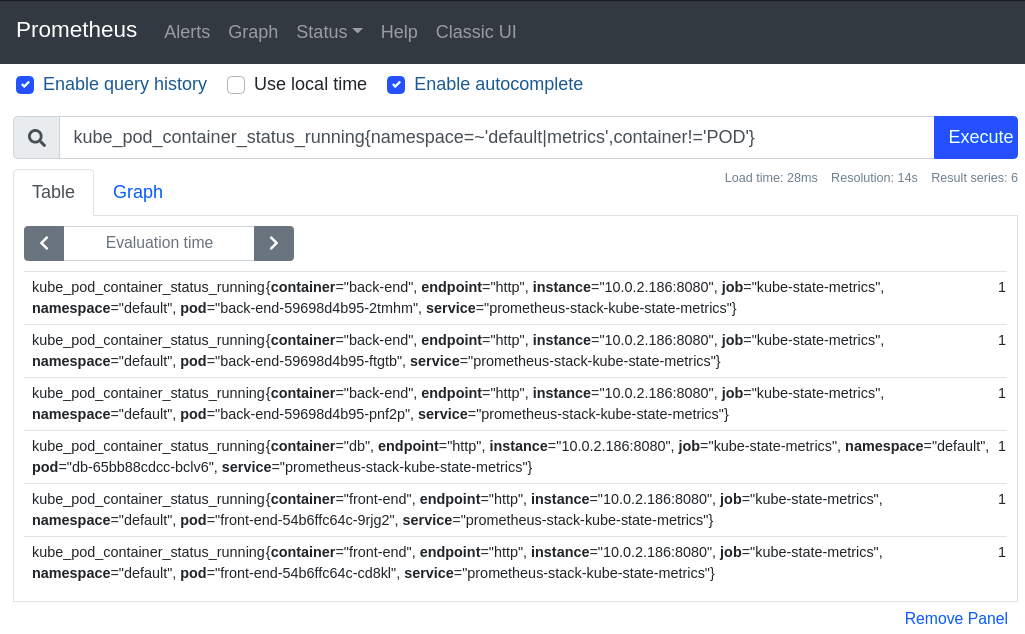
\includegraphics[width=150mm, keepaspectratio]{figures/prometheus_example.png}
\caption{Telepített \textit{Prometheus} rendszere}
\label{fig:prometheus_example}
\end{figure}

Az aktuális rendszerben az operátor még nem külön konténerként fut egy kapszulában, hanem a klaszteren kívül, lokálisan a szerveren, mint egy Go alkalmazás. Emiatt külön telepíteni kellett a Go nyelvet is, hogy el tudjon indulni a rendszer.

\subsection{Verziók}
%----------------------------------------------------------------------------
A rendszer és mérések összeállításához sok különböző komponenset kellett integrálni. Az \ref{tab:versions} táblázat összefoglalóan tartalmazza az egyes környezetek és használt eszközök verzióit. 

\begin{table}[ht]
\centering
  \begin{tabular}{l l}
	  Szoftver 		& Verzió \\
    \hline
      Go 			& 1.16.3 \\ 
      Kubernetes 	& 1.21.0 \\ 
      Kubectl 		& 1.21.0 \\
      Cilium 		& 1.9.5 \\
      Python 		& 3.7.3 \\ 
      Prometheus 	& 2.24.0 \\ 
      Grafana 		& 7.5.3 \\ 
      Operator-SDK 	& 1.4.0-32 \\ 
      Debian 		& 10 (buster)  \\ 
      Istio			& 1.11.4 \\
  \end{tabular}
  
  \caption{Használt verziók}
\label{tab:versions}
\end{table}


%----------------------------------------------------------------------------
\section{Eredmények kiértékelése}
%----------------------------------------------------------------------------
Az egyes méréseknek a kimenete egy-egy \textit{json} fájl, azonban ebből nem nagyon tudunk használható következtetéseket kiolvasni. Szükségessé vált egy külön alkalmazás implementálása, ami az általunk elkészített mérések eredményét fel tudja dolgozni. 

A feladat megoldására szintén a Python nyelvet választottam, mert könnyen lehet benne a \textit{json} objektumokat beolvasni és feldolgozni.
Fontos szempont volt, hogy minél könnyebben használható legyen az alkalmazás, így bizonyos paramétereket akár parancssorban is meg lehet adni. Ez látható az \ref{python_drawer} kódrészleten. Indításnál megadhatjuk, hogy milyen nevet szeretnénk a grafikonnak, milyen címke legyen az $X$ és $Y$ tengelyeken, hogy le akarjuk-e menteni az ábrát, illetve a legfontosabb, hogy melyik mappában keresse a mérési eredményeket. Egy példa konfiguráció is látható a korábban hivatkozott kódrészlet alján. \\

% Rajzoló program indítása --------------------------------------------------
\lstset{caption=Eredményeket feldolgozó alkalmazás használata, label=python_drawer}
\lstinputlisting{figures/python-drawer.sh}

Az alkalmazás indításakor meg kell adni, hogy hova vannak mentve a korábbi mérések során készült kimeneti fájlok. Itt egy-egy mérés jelentése, hogy a Fortio adott darabszámú lekérdezést generál másodpercenként fix ideig. Tehát egy teszteset futtatása több ilyen értelemben vett mérést tartalmaz, hiszen egy skálán megy végig a rendszer, ahol a minimális QPS értéktől megadott lépésközzel halad a maximális QPS értékig. 
Egyesével elkezdi beolvasni a mérési eredményeket és minden fájlból készít egy "tisztázott" eredményt. Ebben már csak az adott grafikon kirajzolásához nélkülözhetetlen értékeket tartalmazza. Például előfordul, hogy a Prometheus eredményében szerepel olyan pod is, ami nem vett részt az adott mérésben, mert még a korábbiból maradt ott. Az ilyen eseteket észlelni kell és kiszedni az értékeit, ne okozzanak anomáliákat. 

%----------------------------------------------------------------------------
\section{Példa mérés}
%----------------------------------------------------------------------------
A rendszer összeállítása után méréseket is lehet már végezni. A mérés mérésben két szolgáltatás vett rész, ahogy az az \ref{fig:sample_sg} sorszámú ábrán is látszik. A szolgáltatáshálóban két különböző feladatot ellátó szolgáltatás szerepelt. Volt egy nodeport segítségével kintről elérhető \textit{front-end} szolgáltatás, illetve egy csak bentről elérhető \textit{back-end}. Azt a szituációt vizsgáltuk, amikor a \textit{front-end} nem használ sok erőforrást, és két pod fut belőle. Ezzel szemben a \textit{back-end} egy jóval erőforrásabb szolgáltatás, cserébe három egység fut belőle. A \textit{front-end} minden felé érkező, \verb+/to-backend+ végpontra érkező kérést továbbított a \textit{back-end} \verb+heavy+ végpontjára. Ezzel elértük, hogy a második szolgáltatásunk a számára beállított, sok processzort igénylő műveletet hajtsa végre.


% Példa szolgáltatás háló----------------------------------------------------
\begin{figure}[!ht]
\centering
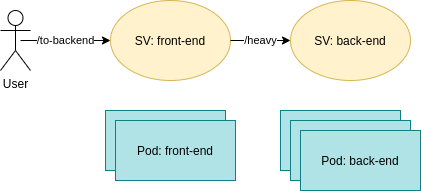
\includegraphics[width=100mm, keepaspectratio]{figures/sample_measurement.png}
\caption{A mérésnek kitett szolgáltatások kapcsolata}
\label{fig:sample_sg}
\end{figure}

A kapott eredményekből készült grafikon látható az \ref{fig:example_plot} és \ref{fig:example_responsetime} ábrán. 

A kapott \ref{fig:example_responsetime} ábráról leolvasható, hogy az átlagos válaszidő a mérés során nem változott érdemben, végig kellően alacsony maradt. Fontos megjegyezni, hogy a mérés során nem vittünk a rendszerbe mesterséges késleltetést, csak a kötelező műveletek elvégzését vártuk meg, így jött ki az állandó válaszidő.

A másik, \ref{fig:example_plot} grafikonon látható, hogy a kevésbé erőforrás-igényes \textit{front-end} processzor felhasználása lassan de folyamatosan nő egészen addig, amíg a \textit{back-end} is tudja növelni a processzor felhasználását. Ez körülbelül 125 QPS-ig tart. Ilyenkor a \textit{back-end} eléri az indításkor beállított erőforrás limitációt és emiatt nem tud több beérkező igényt kiszolgálni.  Emiatt a felhasználói forgalmat generáló Fortio sem fog tudni több kérést a rendszer felé küldeni, mert meg kell várja, mire a \textit{front-end} válaszol, de a front-end csak azután válaszol, hogy meghívta a végletekig megterhelt \textit{back-end} szolgáltatást.

Érdemes figyelembe venni, hogy az $X$ tengely az igényelt lekérdezések darabszámát mutatja, nem a rendszer által valóságban kiszolgált kérések mennyiségét. \\


% Generált példa ábrák -------------------------------------------------------
\begin{figure}[!ht]
\centering
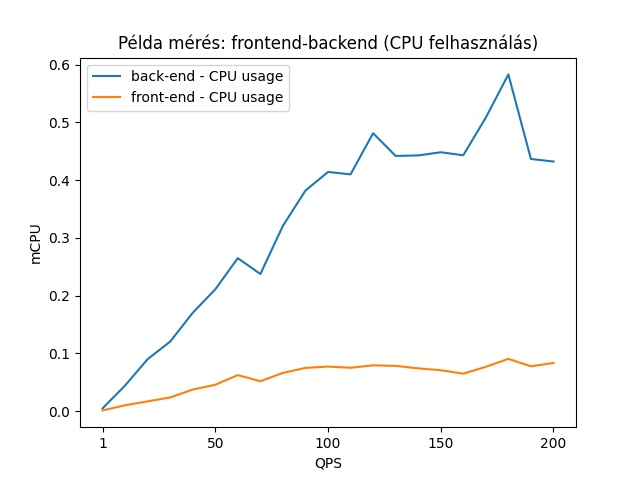
\includegraphics[width=150mm, keepaspectratio]{figures/sample_plot_cpu.jpg}
\caption{\textit{Front-end} és \textit{back-end} egységből álló rendszer CPU felhasználása}
\label{fig:example_plot}
\end{figure}

\begin{figure}[!ht]
\centering
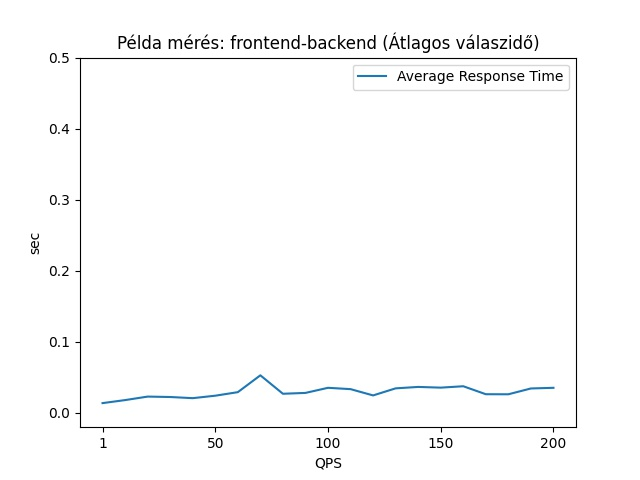
\includegraphics[width=150mm, keepaspectratio]{figures/sample_plot_responsetime.jpg}
\caption{\textit{Front-end} és \textit{back-end} egységből álló rendszer átlagos válaszideje}
\label{fig:example_responsetime}
\end{figure}


%----------------------------------------------------------------------------
\section{Finomhangolás}
%----------------------------------------------------------------------------
% TODO: frissíteni / törölni
Az eredmények megjelenítésén még lehetne finomítani, mivel jelenleg egy grafikonon csak egy mérési sorozat kimenetét dolgozzuk fel. Ez viszont azzal jár, hogy az egyes mérések során lehetségesek eltérések. Például ilyen lehet, hogy a Prometheus még nem tudta lekérdezni az összes konténer utolsó erőforrás-használatait. A probléma orvoslására jelenleg biztonsági időket iktattunk be a mérés során, hogy minimalizáljuk ennek az esélyét. A szebb megoldás viszont az lenne, ha több mérést végeznénk azonos feltételek mellett és ezeknek az átlagát vennénk figyelembe.

Illetve érdemes elgondolkodni, hogyan kellene kezelni az esetet, ha a rendszer nem tudja kiszolgálni az elvárt lekérdezéseket. Több megoldás is szóba jöhet. Egyik, hogy már a mérések végzése folyamán figyeljük és ha nem tudja teljesíteni, akkor idő előtt leállítjuk a terheléseket. Másik, hogy az $X$ tengelyen a valódi, kiszolgált QPS értéket jelenítjük meg. Ezzel annyi gond lehet, hogy elveszítjük az információt, hogy az adott mérésnél a rendszer már túlterhelt állapotban volt és emiatt vagy alapból ennyi kéréssel terheltünk. Harmadik megoldás, hogy az $X$ tengelyen lévő értékeket addig ábrázoljuk, amíg elvárt módon futottak a mérések.

Másik apróság, ami segítene az eredmények vizualizációjában, ha a felhasznált erőforrások és a hozzá kapcsolódó válaszidő egy ábrán lenne, viszont ehhez külön $Y$ tengely fog kelleni, hiszen más a mértékegysége.  

%----------------------------------------------------------------------------
\section{Tervezett mérések}
%----------------------------------------------------------------------------
A korábban bemutatott eredmények alapján a rendszerrel képesek vagyunk méréseket végezni az elvárt módon. Egyenlőre a kapott eredményekből még nem lehet nagyobb következtetéseket levonni, azonban segítség volt megtervezni a következő mérések környezetét. 

Jelenleg a Fortio az alapbeállításokkal indul el, ami 4 felhasználót szimulál. Emiatt tapasztaltuk az, hogy miután a \textit{back-end} telítésbe ment nem érkezett a \textit{front-end} felé több lekérdezés ami tovább tudta volna használni az erőforrásokat.  Szerencsére a könnyen módosíthatjuk ezt a beállítást és tetszőleges számú felhasználót (thread) tudunk majd szimulálni. Érdemes lehet majd ezt is külön paraméterként kivezetni a mérés konfigurációjába.

\begin{itemize}
\item \textbf{1 front-end, 1 back-end, 1 thread} - Ez lenne a legegyszerűbb eset. Később össze lehet hasonlítani a komplexebb mérési környezetekkel.
\item \textbf{1 front-end, 1 back-end, ~100 thread} - Várhatóan érdekesebb eredményeket fog hozni, mert ebben az esetben hiába lesz telítésben a \textit{back-end} a \textit{front-end} még fogadni fogja a többi felhasználó kéréseit, ami így várhatóan a \textit{back-end} előtt fel fog torlódni.
\item \textbf{Előző mérések, csak proszesszorigényes front-end} - Az előző méréseket meg lehet ismételni, csak más szolgáltatáshálón. Ebben az esetben a \textit{front-end} lenne az erőforrásigényes és a \textit{back-end} a könnyen kiszolgálható. Ebben az esetben már a \textit{front-end} előtt el kell dobódni a lekérdezéseknek.
\item \textbf{Horizontális skálázóval} - Miután megvannak a fenti mérések el tudjuk dönteni, hogy milyen eseteket érdemes megismételni és kiegészítve a horizontális pod skálázóval.
\end{itemize}

%----------------------------------------------------------------------------
\section{Elvégzett mérések}
%----------------------------------------------------------------------------
A projektmunka jelentős részét tette ki, hogy méréseket kellett végezni a korábban bemutatott rendszerelelmekkel rendelkező környezetben.
A mérések darabszámát szemlélteti \aref{python_drawer} kódrészlet. Beépített Linux parancsok segítségével könnyen megkaphatjuk a projekt során készített és a kiértékeléshez használt \textit{json} dokumentumok darabszáma. Ahogy a kódrészlet is mutatja először rekurzívan lekérdezzük az adott mappán és almappákon belül található adott kiterjesztéssel rendelkező fájlokat \textit{(find)}. 
Majd az így kapott eredményt csővezeték segítségével hozzákötjük egy szintén beépített parancs \textit{(wc)} bemenetére, ami megszámolja a kiírt sorok számát. 
Ahogy az a kódrészleten is látszik, hogy ennek a kimenete $1445$, ami azt jelenti, hogy a projekt jelenlegi állapotához kapcsolódóan ennyi mérés született. %TODO konkrét mérési számot frissíteni
Az egyes mérések itt egy-egy Vegeta terheléshez kapcsolódó konfigurációk, válaszidők és egyéb Prometheus-ból kapott eredményeket jelenti.

% Mérések számának meghatározása --------------------------------------------
\lstset{caption=Elvégzett mérések száma, label=number_of_measurements}
\lstinputlisting{figures/get_number_of_measuremnts.sh}

\subsection{Költséghatékony frontendek és költséges backend láncban}
\label{subsec:3FE_1BE_chain}
%----------------------------------------------------------------------------
A konkrét mérése előtt is kíváncsiak voltunk, hogyan viselkedik a rendeszer abban a helyzetben, ha több költséghatékony alkalmazáson keresztül jut el egy erőforrásigényes hátsó alkalmazáshoz.
A szinumlált szolgáltatáshálót alkotó elemek \aref{tab:3FE_1BE_chain} táblázatban bemutatott specifikációkkal rendelkeznek.
Látható, hogy a három költséghatékony frontend, egymásnak továbbítják a beérkező kéréseket.
Jelen állásban a könyebbség nevében mindegyikből egy darab replika fut, azonos paraméterekkel. 
Egy-egy kérés kiszolgálása nagyjából 10mCPU processzort igényel, és 1000mCPU volt a lefoglalt és a frontendek által felhasználható erőforrás mennyisége is. Ezek alapján $\frac{1000 mCPU}{10 mCPU/kérés} = 100 kérés$ kiszolgálására elegendő erőforrás van számukra allokálva.
Ezzel szemben, a sor végén álló, költséges backend maximum 2vCPU-t használhat, és az egyes beérkező lekérdezések kiszolgálására 100 mCPU processzorra van szükségük. Ebből kifolyólag maximum $\frac{2000 mCPU}{20 mCPU/kérés} = 20 kérés$ kiszolgálására van lehetőség másodpercenként. 

Minden kérés a \textit{front-end-1}-hez érkezik be és innen kerül továbbításra. Mivel a sor elején lévő egységek ötször több kérést tudnak kiszolgálni, ezért a szűk keresztmetszet a sor hátulján lévő \textit{back-end-1} lesz. Emiatt minden kérésnek el kell jusson a sor végére, miközben az előtte lévő egységek miatt használja az erőforrásokat és mire a sor végére eljut és feldolgozásra kerül, addig a beérkező \textit{http} kapcsolat eldobásra is kerül a beállított öt másodperces időkorlát miatt.

\begin{table}[ht]
\centering
\begin{tabular}{l|llll}
Név                                                            & front-end-1    & front-end-2    & front-end-3   & back-end-1 \\ \hline
Replikák száma                                                 & 1              & 1              & 1             & 1          \\
\begin{tabular}[c]{@{}l@{}}CPU használat\\ (mCPU)\end{tabular} & 10             & 10             & 10            & 100        \\
\begin{tabular}[c]{@{}l@{}}CPU limit\\ (mCPU)\end{tabular}     & 1000           & 1000           & 1000          & 2000       \\
\begin{tabular}[c]{@{}l@{}}Memória limit\\ (kB)\end{tabular}   & 1000           & 1000           & 1000          & 1000       \\
Továbbhívás                                                    & front-end-2:80 & front-end-3:80 & back-end-1:80 & -         
\end{tabular}
  	\caption{Három költséghatékony frontend után egy költséges backend}
	\label{tab:3FE_1BE_chain}
\end{table}

Az ismertetett környezetben elvégzett mérésről készített grafikon látható \aref{fig:3FE_1BE_chain} ábrán.
Megfigyelhető, hogy az egyre nagyobb beérkezett terhelés hatására folyamatosan növekszik a rendszer által felhasznált erőforrások mennyisége.
Különösen érdekes, hogy a \textit{back-end-1} által használt processzor mennyisége, a várt módon, 20 lekérdezés / másodperc érték környékén eléri a maximumot, onnan már nem emelkedik továss, csak stagnál. 
Ezzel ellentétben az egyes frontend alkalmazások erőforrásigénye folyamatosan növekszik a mérés végéig.

Ezzel párhuzamosan a memória használata is érdekesen alakul.
18 QPS értékig látszólag nem változik éredmben, alacsonyan marad.
Azonban a backend telítése után, minden egységnél elkezd növekedni.
Ez azzal magyarázható, hogy a rendszerben lévő várakozási sorok, bufferek folyamatosan telnek meg, mivel a láncolat végén lévő költséges backend nem képes a beérkezések számával tartani a kiszolgálási számot. 
%TODO: Markow láncok / tömegkiszolgálással magyarázni.  http://www.szit.bme.hu/~gyorfi/tomkisz.pdf

Az alsó sorban látható grafikonok segítségével leolvasható, hogy az átlagos válaszidők 20 QPS környékén elérik az 5 másodperces felső korlátot, amivel szinkronban az időben kiszolgálásra kerülő kérések száma is drasztikusan elkezd visszaesni, majd utána a beérkező kérések elhanyagolható részét tudjuk csak időn belül kiszolgálni. 
Összeségében megállapítható, hogy létezik egy olyan pont a szimulációban, aminél több beérkező kérés esetén csak az erőforrásokat használjuk és az érdemi kiszolgálás is hirtelen és drasztikus mértékben visszaesik.
Ilyenkor elszállnak a késleltetések és memória használat, valamint folyamatosan nő a processzor használata is.

\begin{figure}[!ht]
	\centering
	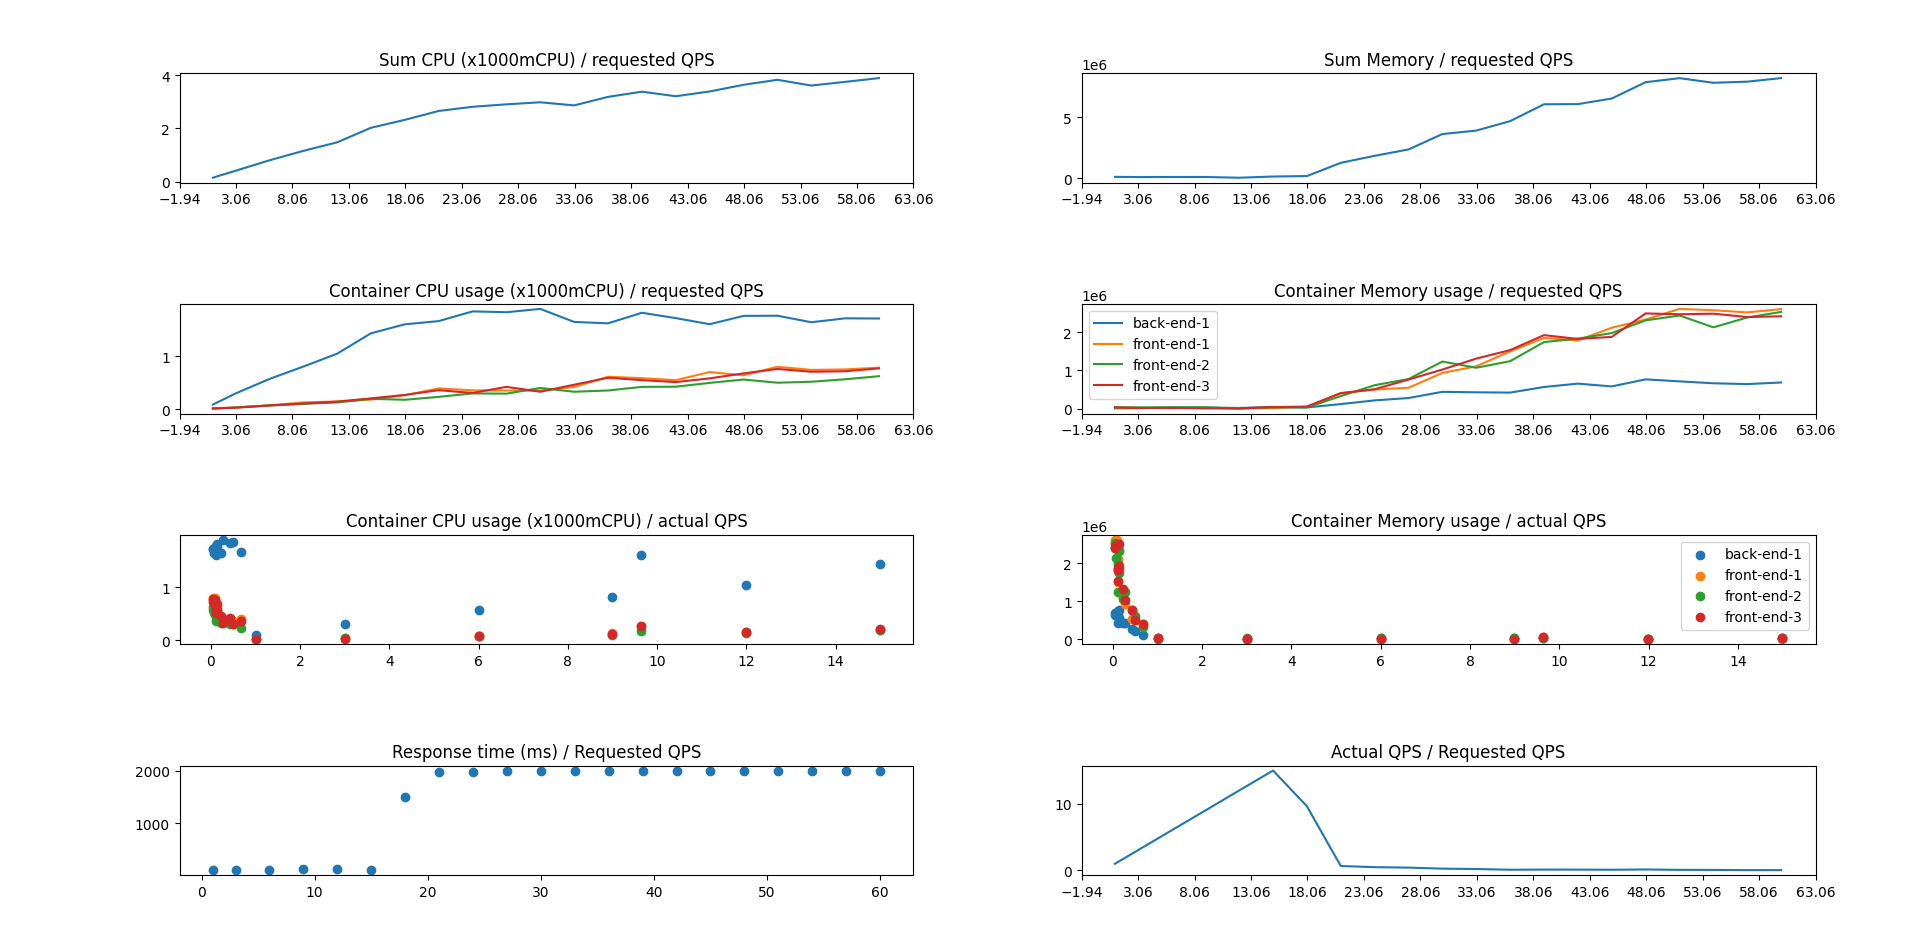
\includegraphics[width=150mm, keepaspectratio]{figures/taildrop-chain-3FE-1BE_requestedQPS.png}
	\caption{Három költséghatékony frontend után egy költséges backend mérés ábrázolása}
	\label{fig:3FE_1BE_chain}
\end{figure}

\subsection{Költséghatékony frontendek egymás mellett és költséges backend mögöttük}
%----------------------------------------------------------------------------
\Aref{subsec:3FE_1BE_chain} fejezetben bemutatott tapasztalatokat igazoló, készítettem egy következő mérést is. Ebben az esetben kicsit egyszerűbb architektúrával végeztem el a mérést. A megkonstruált erőforráshasználatok és a rendszer felépítését táblázatos formában \aref{tab:3FE_1BE_new} táblázat tartalmazza.

Fontos különbség, hogy ebben a mérésben nem hozunk létre egy hosszú láncot az egyes frontend alkalmazások egymás mögé kötésével, hanem ennél sokkal rövidebb lesz egy-egy kérés kiszolgálásának folyamata. 
A költséghatékony frontend után rögtön a költséges backendhez kerül továbbításra a beérkező kérés.
Ezen kívül még egy fontos módosítás, hogy három darab frontend fog futni és továbbra is egy backend lesz hátul.
A megadott alapján kiszámolható az egyes egységek által körülbelül kiszolgálható kérések száma másodpercenként.
\refstruc{eq:3FEsumqps} alapján leolvasható, hogy a \textit{front-end-1} áteresztő képessége 120 kérés, míg a \textit{back-end-1} ennél jóval szerényebb 20 beérkező kérést tud kiszolgálni másodpercenként, mint ahogy az következik \aref{eq:1BEsumqps} egyenletből.

\begin{equation}
\label{eq:3FEsumqps}
3(replika)\times\frac{1000 mCPU}{25 mCPU/kérés} = 120 kérés/másodperc
\end{equation}

\begin{equation}
\label{eq:1BEsumqps}
1(replika)\times\frac{2000 mCPU}{100 mCPU/kérés} = 20 kérés/másodperc
\end{equation}

\begin{table}[]
\centering
\begin{tabular}{l|ll}
Név                                                            & front-end-1   & back-end-1 \\ \hline
Replikák száma                                                 & 3             & 1          \\
\begin{tabular}[c]{@{}l@{}}CPU használat\\ (mCPU)\end{tabular} & 25            & 100        \\
\begin{tabular}[c]{@{}l@{}}CPU limit\\ (mCPU)\end{tabular}     & 1000          & 2000       \\
\begin{tabular}[c]{@{}l@{}}Memória limit\\ (kB)\end{tabular}   & 1000          & 1000       \\
Továbbhívás                                                    & back-end-1:80 & -          \\
HPA                                                            & -             & -         
\end{tabular}
  	\caption{Költséghatékony frontend több replikával és utána egy költséges backend}
	\label{tab:3FE_1BE_new}
\end{table}

Jelen mérésben nincsen megadva semmilyen automatikus skálázó, ezért amikor az operátor az indításkor létrehozza adott replikaszámmal az egyes Kubernetes Deploymenteket, azok nem is fognak változni, függetlenül a beérkező kérések mennyiségétől.
A korábban bemutatott környezeten is elvégeztem a szimulált terheléssel történő mérést.
Ezen eredményeket mutatja be \aref{fig:3FE_stack_1BE} ábra.
A korábbi méréssel szinkronban, hasonló megállapításokat tudunk leolvasni.
Látható, hogy a \textit{back-end-1} telítése az elvárt 20 QPS körül megtörténik (illetve kicsit még előtte). 
Azonban ettől függetlenül a \textit{front-end-1} által elhasznált processzor mennyisége folyamatosan nőtt. A legmagasabb terhelésnél már olyan szintre emelkedett a három példány által összesen használt processzor erőforrása, mint a backend maximuma, tehát mintha 2 teljes virtuális CPU magot is allokáltunk volna számukra.

A költséges backend telítése után jelentősen megugrik a beérkező kérések kiszolgálásához szükséges késleltetések és az egyes egységek által használt memória mennyiségek is.
A jobb alsó grafikonon látszik, hogy 20 QPS-nél már vissza is zuhant a sikeres kiszolgálások száma, amivel szinkronban a kiszolgálások átlagos válaszideje is felurik a maximumra, ami jelenleg 5 másodperc, mert a beállítások szerint ennyi idő után bontjuk a \textit{http} kapcsolatokat.

\begin{figure}[!ht]
	\centering
	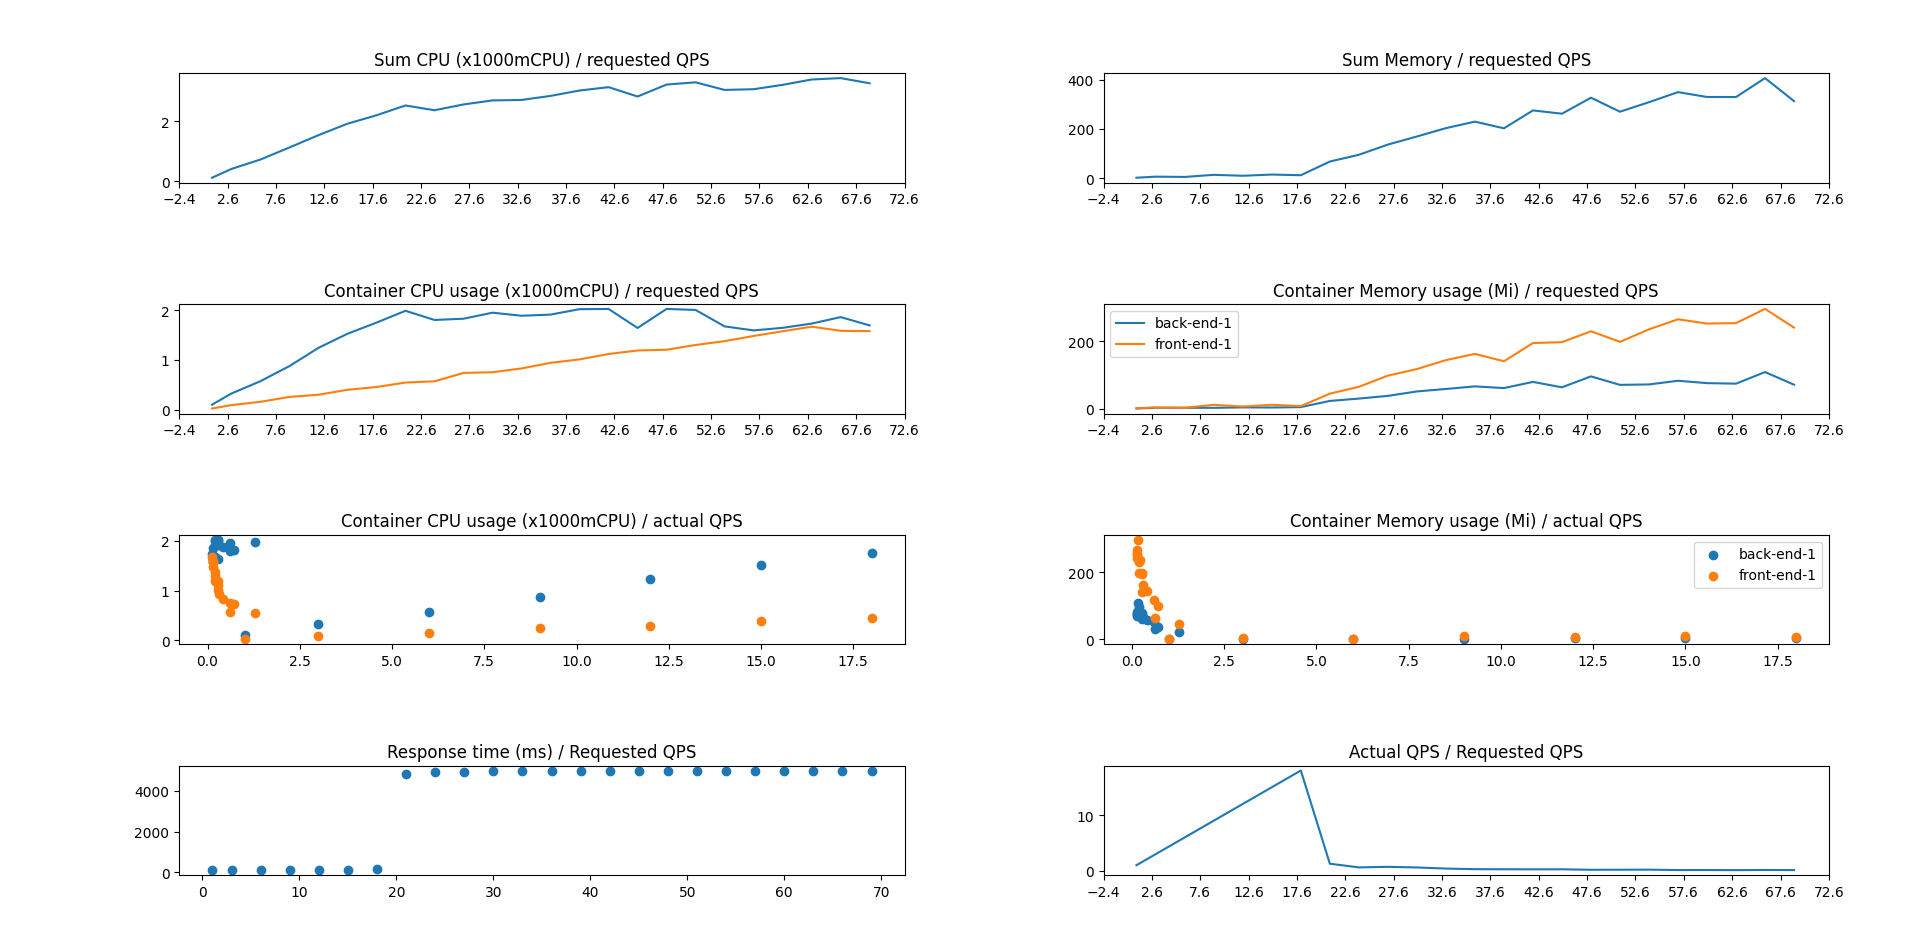
\includegraphics[width=150mm, keepaspectratio]{figures/multiFE-singleBE.png}
	\caption{Költséghatékony frontend három példányban és utána egy költséges backend mérés ábrázolása}
	\label{fig:3FE_stack_1BE}
\end{figure}

Röviden elmondható, hogy a beérkező kérések növekedésével együtt fokozatosan nő az elhasznált processzor mennyisége és a sikeres kiszolgálások száma is.
Azonban van egy pont, amikor a hálózatban lévő szűk keresztmetszet nem képes tartani a lépést a beérkező kérések mennyiségével. 
Ebben az esetben hirtelen visszaesik a kiszolgálás minősége, drasztikusan megugrik a várható kiszolgálási idő és ezzel együtt csökken a sikeres kiszolgálások aránya.

Az elvégzett mérések esetén látható, hogy valódi problémáról van szó, abban az esetben, ha a rendszer az előre definiált erőforráshasználatokkal fut és nem képes azokat automatikusan állítani.
Ha a beállítások dinamikusabbak lennének, akkor például a frontend által lefoglalt és használt erőforrásokat át lehetne csoportosítani a backend részére, amivel növelhető lenne a rendszer globális maximum kiszolgálása.

%----------------------------------------------------------------------------
\section{Mérések automatikus horizontális skálázóval}
%----------------------------------------------------------------------------

A korábban végzett mérések alapján ki lehet jelenteni, hogy a podok statikus konfigurálásával nem mindig találjuk meg a rendszer ideális állapotát,  sőt a jövőbeli terhelés pontos információja nélkül nagyon valószínű, hogy szuboptimális állapotban maradunk.
A Kubernetes beépítetten támogatja a podok automatikus horizontális skálázását, mint ahogy azt \aref{subsec:hpa} alfejezetben bemutatásra került.
A további haladás részeként szerettem volna megnézni, hogy milyen megoldást kínál beépített skálázó és mik a limitációi.
A fő cél az volt, hogy bizonyítást nyerjen, hogy a skálázó algoritmusa miatt nem képes minden esetben egy ideális állapotba jutni.

\subsection{Áttérés nehézségei}
%----------------------------------------------------------------------------

Az új fajta mérés több gondot is okozott, tekintve hogy az eddigre bejáratott ábrázoló alkalmazást teljesen át kellett variálni, ugyanis ezen mérések jelentősen mások.
Ebben az esetben az egyes értékek az időtől változóan függnek, ellentétben a HPA nélküli méréseknél, amikor minden a beérkező terheléstől változott. Valamint a kezdeti méréseknél kiderült, hogy az elkészített operátor logikai működésében is hiba van. 
A jelenség onnan fakadt, hogy minden egyes alkalommal, amikor az operátorunk futásra került, ellenőrizte a ServiceGraph konfigurációban megadott replika számot és ha nem stimmelt, akkor módosította azt.
Ezen logika miatt, amikor a skálázó szeretett volna több azonos podot elindítani egy adott alkalmazásból, akkor ezt észrevette az operátor és visszaállította a kezdeti értéket.
A következmény pedig az lett, hogy a rendszer sosem került stabil állapotba és skálázó döntései nem tudtak érvényre jutni.

A fenti probléma ideálisan példaként tud szolgálni az operátorok egy kevésbé kutatott és ritkán tárgyalt kihívására.
Amennyiben több kezelő alá esik egy-egy Kubernetes erőforrás, akkor nagyon körültekintően kell eljárni az egyes feladatkörök elosztásában.
Nem triviális észrevenni, ha direkt vagy indirekt módon, egymás döntéseire reagáltan futnak le az operátorok algoritmusai.
Ezzel a rendszer egésze könnyen instabil vagy holtponti (deadlock) állapotba tud kerülni.

Egy-egy ilyen helyzetet felismerni aránylag körülményes, alapértelmezetten nincsen erre külön logika implementálva az orkesztrációs platformba.
Emiatt ezen esetek detektálása, újabb operátor bevonása nélkül nem lehetséges.
Azonban újabb logika bevonása, ami azonos erőforrások kezelését teszi lehetővé, tovább növelheti az indirekt egymásrahatások valószínűségét.

Természetesen a fenti probléma könnyen javíthatónak bizonyult és csak egy kisebb módosításra volt szükség.
Végleges implementációban a megadott replikaszám ellenőrzése az egyes deploymentekben csak akkor kerül ellenőrzésre, ha autómatikus skálázó nem került definiálásra a megadott konfiguráció alapján.

\subsection{Lokálisan mohó, globálisan nem optimális}
%----------------------------------------------------------------------------

% TODO: x. fejezetben bemutatott
A HPA skálázó döntési mechanizmusát ismerve, sejthető volt, hogy milyen szituációkra viselkedhet érzékenyen.
Maga az algoritmus, ami meghatározza az egyes podokból aktuálisan szükséges darabszámot egyedül az ő feleőssége alá tartozó konténereket veszi számításba.
Ezen kívül nem rendelkezik egyéb ismerettel a többi szolgáltatást illetően.
Például nem tudja, hogy milyen más alklamazás komponensekkel van kapcsolatba az alá tartozó komponens se azt, hogy mennyi erőforrás érhető el összesen a klaszterben.

A fenti tulajdonságok alapján a jelenlegi skálázó csak lokálisan optimális döntéseket tud hozni egy-egy alkalmazás egység számára.
Azt kellett bebizonyítani, hogy ezen tulajdonsága miatt a rendszer összeségét érintő, globális optimumot nem fogja megtalálni.
Ehhez létrehoztam egy egyszerű szolgáltatás hálót és az egyes elemekhez tartozó horizontális skálázót. 
A konkrét értékeket \aref{tab:1FE_1BE_chain_with_HPA} táblázat tartalmazza.
Látható, hogy a korábbi mérésekhez hasonlóan itt is egy Frontend és egy Backend alkalmazás szerepel. 
A kérések a frontendhez érkeznek be, ami mindegyiket továbbítja a backend felé. 
Az egyes komponens podok által lefoglalt és maximálisan használható erőforrások mennyisége megegyezik.
Egy virtuális CPU magot használhatnak illetve egy megabájt memóriát.
Annyi különbség van, hogy a frontend a beérkező kérésenként negyed annyi CPU használatot fog generálni, mint a backend.

A korábbi mérésektől eltérően ebben az esetben az operátorunk a konfiguráció alapján fog létrehozni automatikus horizontális skálázót is.
Azonos szabályok kerültek alkalmazásra a két egységhez kapcsolódóan.
Legalább egy podnak futnia kell de legfeljebb öt futhat egyszerre, illetve a processzor használtságot figyelembe véve fogjuk meghozni a skálázási döntést.
Ebben az esetben a HPA törekedni fog a 70 százalékos foglaltságra. 
Tehát a maximálisan elérhető proszeszor használat 70 százaléknál magasabb használata esetén fogjuk megkezdeni a felskálázást.

\begin{table}[]
\centering
\begin{tabular}{ll|ll}
\multicolumn{2}{l|}{Név}                                                                      & front-end-1   & back-end-1 \\ \hline
\multicolumn{2}{l|}{Kezdeti replika szám}                                                     & 1             & 1          \\
\multicolumn{2}{l|}{\begin{tabular}[c]{@{}l@{}}CPU használat\\ (mCPU)\end{tabular}}           & 25            & 100        \\
\multicolumn{2}{l|}{\begin{tabular}[c]{@{}l@{}}CPU foglalás és limit\\ (mCPU)\end{tabular}}   & 1000          & 1000       \\
\multicolumn{2}{l|}{\begin{tabular}[c]{@{}l@{}}Memória foglalás és limit\\ (kB)\end{tabular}} & 1000          & 1000       \\
\multicolumn{2}{l|}{Továbbhívás}                                                              & back-end-1:80 & -          \\
\multirow{3}{*}{HPA}                            & Minimum replika                             & 1             & 1          \\
                                                & Maximum replika                             & 5             & 5          \\
                                                & Cél CPU használat                           & 70\%          & 70\%      
\end{tabular}
\caption{Három költséghatékony frontend után egy költséges backend}
\label{tab:1FE_1BE_chain_with_HPA}
\end{table}

A generált terhelés hatására a rendszernek másodpercenként hetven beérkező kérést kellett kiszolgálnia. 
Az egyes http kapcsolatokra a megszokott módon öt másodperces időkorlát volt, amin belül ha nem érkezett válasz, akkor az adott kérést sikertelennek tekintjük.
A teljes szimuláció a szolgáltatásháló létrehozásától számított tíz percig, azaz hatszáz másodpercig tartott.

Mérés során parancssorból is jól látható a skálázó működése. 
Ezt mutatja be \aref{hpa_measurement_pending} kódrészlet, amin belül két paranccs kimenetét is láthatjuk a mérés kezdetét követő bő öt és feledik percben.
Első sorban lekérdezzük az éppen működésben lévő horizontális skálázókat. 
A parancs kimenetének második oszlopából kiderül, hogy az egyes skálázók az azonos névvel rendelkező deployment erőforráshoz vannak kapcsolva.
Leolvasható, hogy skálázó döntései alapján öt és négy replikának kellene futni ebben az időpillanatban illetve, hogy mind a frontend mind pedig a backend túl lépte a számára előirányzott processor fogyasztást.

A kódrészlet második parancsán láthatjuk, hogy milyen podok és milyen állapotban léteztek ilyenkor.
Megfigyelhető, hogy valóban szerepel a korábban a skálázó által meghatározásra kerülő négy darab frontend és az öt darab backend kapszula.
Viszont, ami tanulságos, hogy közüllük nem mindegyiknek sikerült az elvárt módon elindulnia.
Erre abból lehet következtetni, hogy egyes podok állapot mezője nem az elvárt \textit{Running}, hanem \textit{Pending} állapotban vannak.
Amiatt van ez, mert ugyan a skálázó döntése alapján el kellene induljon az elvárt számú kapszula, azonban a Kubernetes ütemezője nem tudja őket elindítani.
Látható, hogy három plusz három kapszula tudott rendesen elindulni, így rögtön hat virtuális cpu magot le is foglaltunk a klaszterben és nem tud új egységet lehelyezni.
Ez a magyarázata, hogy míg a korábban elindított egységek (magasabb \textit{AGE} értékkel) sikeresen elindultak, azonban a későbbieknél ez már nem mondható el.

% HPA bekapcsolva, nem ideális eredmény ----------------------------------------
\lstset{caption=Horizontális skálázóval történő mérés, label=hpa_measurement_pending}
\lstinputlisting{figures/HPA-pending-pods.sh}

A mérés eredményeit ábrázolva előkerült egy érdekesség is, amit \aref{fig:HPA-scaling-same-time} ábrán láthatunk.
A grafikonon egyszerre van ábázolva a frontendből és a backendből futó egységek száma is.
Erre utal a bal felső sarokban szereplő jelmagyarázat is, viszont a kék színnel rajzolt költségesebb backend nem is látszik.
Ez amiatt van, mert a Prometheus adatai szerint egyszerre történtek meg a skálázások és ez az oka, hogy mindkét alkalmazásegységből három, három darab került elindításra.
Értelemszerűen ez az erőforrások nem ideális elosztását vonja magával, hiszen azonos erőforrás került lefoglalásra és használatra a költségesebb illetve könyebb alkalmazásrész részére is.
Ha a skálázó rendelkezne a környezetéről több inforációval, akkor ennél ideálisabb arányban tudna erőforrásokat allokálni.
Például, ha feltesszük, hogy összesen hat pod indítható, akkor előnyösebb lenne egy 2-4 vagy 1-5 megosztás a költségesebb backend javára.
Viszont a tapasztalható megosztással nem tudjuk maximálisan kihasználni a rendszerben lévő erőforrásokat.
Pontosabban mondva kihasználjuk, mert a lefoglalt processzor mennyiségét jelentősen kihasználjuk, azoban a kiszolgálás minősőgén és mennyiségén ez nem látszódik.

\begin{figure}[!ht]
	\centering
	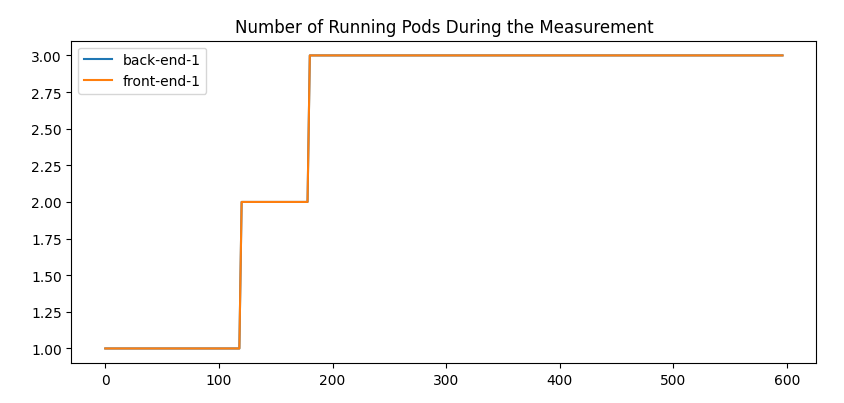
\includegraphics[width=150mm, keepaspectratio]{figures/HPA-scaling-in-the-same-time.png}
	\caption{HPA skálázóval történő mérés}
	\label{fig:HPA-scaling-same-time}
\end{figure}

